\documentclass[12pt, a4paper, oneside, ngerman]{article}
\usepackage[utf8]{inputenc}
\usepackage[T1]{fontenc}
\usepackage[]{hyperref}
\usepackage{graphicx}
\usepackage{listings}
\usepackage{caption}


\title{Projektarbeit Compilerbau}
\usepackage[german]{babel}


\begin{document}
\selectlanguage{german}
\author{Jonas Wenner, Jens Marvin Reuter, Noah Hoffmann}



\maketitle
% * <john.hammersley@gmail.com> 2015-02-09T12:07:31.197Z:
%
%  Click the title above to edit the author information and abstract
%
\thispagestyle{empty}
\pagebreak

\tableofcontents
\newpage


\section{Einleitung}

Als Abschlussprojekt des Moduls 'Compilerbau' unter Leitung von Thorsten Jakobs, M.Sc., htw saar wurde dieser Compiler zur von uns eigens entwickelten Sprache \textit{Team Progbusters Language} (Arbeitstitel) entwickelt, mit den in \textit{2. Anforderungen} beschriebenen Voraussetzungen und Zielen. Die Sprache basiert im Wesentlichen auf C, wurde jedoch auf wesentliche Elemente wie Grundrechenarten, Funktionen, if-Statements und eine Form der Schleife reduziert. Weiterhin vorhanden sind Bezeichner, Konstanten, Variablen, die Klammerung wird ebenfalls ber\"ucksichtigt.


Diese Dokumentation behandelt die Anforderungen an den Compiler, den theoretischen Hintergrund, die Konzeption der Entwicklung, unsere verwendeten Technologien, sowie unsere Vorgehensweise während der Entwicklung und die Probleme, auf die wir gestoßen sind und unsere Lösungsansätze. Ausgangs wird auch die Handhabung des Compilers näher erläutert.

\newpage

\section{Anforderungen}

Um zu gewährleisten, dass alle Modulteilnehmer über die gleichen Vorraussetzungen verfügen und nach festgelegten Kriterien bewertet werden können, wurden durch den Modulverantwortlichen einige Rahmenbedingungen vorgegeben. Die Prüfleistung besteht dabei aus der Entwicklung einer einfachen Programmiersprache, dem Anfertigen einer Dokumentation sowie der Präsentation der Ergebnisse. Die Anforderungen an das Projekt werden in den folgenden Abschnitten aufgeführt und erläutert.

\subsection{Infrastruktur}
Das Ziel ist die Enwicklung eines Frontends, welches Quelltext in der von uns entwickelten Programmiersprache zu Jasmin-Code übersetzt. 
Jasmin ist ein Assembler für die Java Virtual Machine, der Quelltext in einer assembler-artigen Syntax zu Bytecode übersetzt. 
Dieser Bytecode kann schließlich von der Java Virtual Machine ausgeführt werden.


\subsection{Programmiersprache}
Die von uns entwickelte Programmiersprache besitzt folgende Komponenten: 
\begin{itemize}
\item Bezeichner
\item Konstanten (TO BE IMPLEMENTED!)
\item Variablen
\item Arithmetik mit Grundrechenarten
\item Klammerung
\item Funktionen
\item if-else-Anweisung
\item while-Schleife (TO BE IMPLEMENTED!)
\end{itemize}
\noindent
Die Entwicklung wird mit 50\% in der Gesamtbewertung gewichtet.
In einem späteren Kapitel dieser Dokumentation wird erläutert, wie die Programmiersprache verwendet wird.

\subsection{Dokumentation}
Es ist eine Dokumentation anzufertigen, die Aufschluss über die Konzeption der Entwicklung, die verwendeten Technoligen, das Vorgehen während der Entwicklung, aufgetretene Probleme und Lösungsansätze zu diesen sowie die Verwendung des Compilers gibt.

Die Dokumentation wird mit 30\% in der Gesamtbewertung gewichtet.

\subsection{Präsentation}
In einer circa 20-minütigen Präsentation werden die verwendeten Technologien, wichtige Entwicklungsschritte sowie aufgetretene Probleme erläutert. Außerdem wird der Compiler vorgeführt. 

Die Präsentation wird mit 20\% in der Gesamtbewertung gewichtet.

\pagebreak
\section{Theoretischer Hintergrund}
Um die folgenden Abschnitte verständlich zu machen ist eine kurze Erläuterung des theoretischen Hintergrunds sinnvoll.
\subsection{Verallgemeinerung}
Der zu entwickelnde Compiler nimmt als Eingabe eine Text-Datei mit Instruktionen in der Ausgangssprache. Der Compiler verarbeitet diese Eingabe und gibt als Ausgabe eine Datei mit Anweisungen in der Zielsprache zurück. Diese Verarbeitung kann grob in drei Abschnitte eingeteilt werden.
\subsection{Lexikalische Analyse}
Der erste Schritt ist dabei die sogenannte lexikalische Analyse. Die Eingabedatei ist für den Computer zunächst nur eine Kette von Zeichen. Diese Zeichen sind in sogenannte Tokens aufzuteilen. Beispielhaft könnte die Eingabe
\begin{lstlisting} [frame=single]
 a = b + c;
\end{lstlisting}

zu den folgenden Tokens aufgelöst werden.

% @Marvin, pls eine bessere Grafik erstellen. Dankeschön (-:
% @topkek, wird gemacht.
\begin{figure}[h!]
\centering
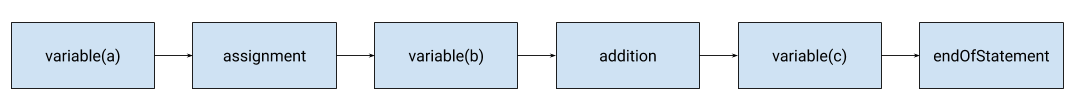
\includegraphics[scale=0.37]{lex_beispiel.png}
\caption{Kurzes Beispiel für lexikalische Analyse}
\label{fig:method}
\end{figure}


Der Teil des Compilers, der diese Aufgabe übernimmt, wird Lexer genannt. Der Lexer überprüft für jedes Zeichen der Eingabedatei, welchem Token dieses zugeordnet werden kann. Dies geschiet auf Grundlage von definierten Regeln, welche mit sogenannten regulären Ausdrücken formuliert werden. Ein regulärer Ausdruck besteht aus einer Sequenz von Zeichen, die ein bestimmtes Muster definieren. Reguläre Ausdrücke können auch rekursiv verwendet werden, um auf Grundlage einfacher regulärer Ausdrücke komplexere zu bilden. Beispiele für reguläre Ausdrücke werden im Kapitel HIER KAPITELNUMMER EINFÜGEN Erste Schritte: Auswertung von arithmetischen Ausdrücken aufgeführt.

\subsection{Syntaktische Analyse}
Der zweite größere Abschnitt besteht in der syntaktischen Analyse. Dabei wird überprüft, ob die Eingabedatei einer definierten Grammatik entspricht. Bei der lexikalischen Analyse wird lediglich die übergebene Zeichenfolge in Tokens aufgeteilt, jedoch nicht überprüft, ob diese der Grammatik entsprechend zusammengeführt werden können. 
Bei einer erfolgreichen Auswertung wird die Folge an Tokens, die bei der lexikalischen Analyse ermittelt wurde, in einen Syntaxbaum übergeführt. Dies ist notwendig, um die Tokens in der richtigen Reihenfolge auszuwerten. 
%hier wäre eine Grafik auch hilfreich

\subsection{Syntaxgesteuerte Übersetzung}
Die eigentlich Erzeugung von Code in der Ausgangssprache findet zuletzt statt. Hierbei wird jeder Knoten des Syntaxbaum betrachtet und je nach Kontext eine Zeichenkette mit Anweisungen in der Zielsprache generiert. In diesem Schritt findet ebenfalls die semantische Analyse statt, beispielsweise die Überprüfung, ob eine aufgerufene Variable vorher deklariert wurde.

\pagebreak
\section{Konzeption der Entwicklung}
\subsection{Allgemeiner Grundsatz}
Während der Entwicklung versuchten wir uns möglichst kleine Zwischenziele zu setzen, um die Aufgabe in überschaubare, einfach zu lösende Teilprobleme zu unterteilen. Rückblickend war dies eine sinnvolle Strategie, die zum gewünschten Ziel führte.

\subsection{Wahl der Entwicklungswerkzeuge}
Bezüglich der Entwicklungswerkzeuge wurden uns verschiedene Möglichkeiten vorgestellt. Die erste Möglichkeit bestand darin das Tool ''lex'' beziehungsweise dessen Open-Source-Implementierung ''flex'' als Lexer-Generator und das Tool ''yacc'' beziehungsweise dessen Open-Source-Implementierung ''bison'' als Parser-Generator zu nutzen. Die zweite Möglichkeit bestand in der Nutzung des Werkzeuges ANTLR, das die Funktionalitäten der zuvor genannten Werkzeuge in einem Programm zusammenfasst.

Da ANTLR automatisiert auf Grundlage einer Datei, die die von uns formulierte Grammatik der Sprache enthält, Lexer sowie Parser zeitgleich erstellen kann, entschieden wir uns für diese Variante. Der Vorteil besteht dabei darin, dass zwei essentielle Teile des Compilers von einem Tool übernommen werden. 

\subsection{Sprachdesign}
Es wurde sich darauf geeinigt, dass die Syntax der von uns entworfenen Ausgangssprache der der Programmiersprache C ähnlich sein soll, da alle Projektteilnehmer mit dieser Sprache vertraut sind und C allgemein weit verbreitet ist.

\subsection{Implementierung}
Unser Compiler verwendet im Zusammenspiel mit dem von ANTLR generierten Lexer und Parser einen Visitor für die syntaxgesteuerte Übersetzung. Die Alternative dazu besteht in einem Listener, der sich von einem Visitor dahingehend unterscheidet, dass die verschiedenen Methoden die auf die Knoten des Syntaxbaumes angewandt werden, keinen Rückgabewert besitzen und die Ergebnisse dieser somit seperat gespeichert werden müssen. Der Vorteil eines Listeners hingegen besteht darin, dass untergeordnete Knoten im Syntaxbaum automatisch bearbeitet werden und nicht wie beim Visitor explizit besucht werden müssen. Nach der Abwägung diser Vor- und Nachteile entschieden wir uns für einen Visitor, da es uns weniger komplex erschien.




\pagebreak
\section{Verwendete Technologien}

\subsection{Eclipse}
Zur Entwicklung wurde die integrierte Entwicklungsumgebung Eclipse Photon in der aktuellesten Version (4.8.0) genutzt. 
Eclipse bietet mehrere Vorteile, die ein einfacheres und effizienteres Entwickeln erlauben. Eclipse enthält einen Datei-Explorer mit dessen Hilfe die Navigation durch die verschiedenen Verzeichnisse im gleichen Fenster wie der Editor und die Konsole geschehen kann. Des Weiteren bietet Eclipse automatische Vervollständigungsvorschläge an, was die Schreibgeschwindigkeit erhöht. 
Außerdem kann Eclipse durch Plug-Ins erweitert werden. Wir nutzten beispielsweise das Testframework TestNG als Plug-In um verschiedene Testfälle automatisiert zu prüfen.

\subsection{TestNG}
TestNG ist ein Framework, dass dem zu testenden Programm Eingabewerte übergeben und die tatsächlichen Ergebnisse des Programms mit erwarteten Ergbnisses abgleicht. Dabei können beliebig viele Testszenarien geprüft werden. Es werden sogenannte positive Tests, also solche bei denen die Eingabe ein vorgehesenes Ergebnis hervorruft, als auch negative Tests, bei denen geprüft wird, ob nicht vorhergesehene Eingaben mit entsprechenden Fehlermeldungen korrekt gehandhabt werden, durchgeführt. TestNG wurde von uns in Version HIERVERSIONEINFÜGEN genutzt.
\linebreak
Als Beispiel: Der Quelltext ''println(1+4);'' sollte als Ergebnis ''5'' auf der Konsole ausgeben. TestNG übergibt den Quelltext an unseren Compiler, ruft Jasmin auf, führt das Programm aus und gleicht dann die Ergebnisse ab. Wenn das Ergebnis ''5'' ist gilt der Test als bestanden, andernfalls als durchgefallen. 

\subsection{ANTLR}
ANTLR steht für ANother Tool for Language Recognition und ist ein Lexer- und Parsergenerator. ANTLR generiert auf Grundlage einer Grammatik-Datei Java-Code, der einen entsprechenden Lexer sowie ein Template für Teile des Parsers implementiert. Dadurch, dass die von ANTLR generierten Programme aus einer Eingabedatei in der Ausgangssprache einen Syntaxbaum erstellen können, liegt unsere Arbeit größtenteils darin Grammatiken für ANTLR zu formulieren und Teile des Parsers (in unserem Fall ein Visitor) zu implementieren. Wir verwendeten die ANTLR-Version 4.7.1.

\subsection{Jasmin}
Jasmin ist ein Assembler für die Java Virtual Machine. Dabei werden Textdateien mit Anweisungen in Jasmin-Syntax zu Bytecode übersetzt. Dieser Bytecode kann von der JVM ausgeführt werden.

\subsection{Java}
Die Programmiersprache Java wurde für das Projekt gewählt, da der von ANTLR generierte Code ebenfalls in Java ist. Es ist teilweise notwendig von Klassen des ANTLR generierten Code abzuleiten, weshalb die Wahl einer anderen Programmiersprache keinen Sinn ergeben hätte. 
Des Weiteren muss die Java Runtime Environment ohnehin genutzt werden, um ANTLR, Jasmin sowie schließlich die Kompilate des HIERNAMEUNSERERSPRACHEEINFÜGEN-Compilers auszuführen.

\subsection{Java Virtual Machine}
Die Java VM ist ein Zwischenschritt beim Ausführen von Java-Code. Eine Java-Quelldatei (.java) wird zunächst durch den Java-Compiler zu Bytecode (.class) übersetzt und dann von der Java VM interpretiert. Dieser Zwischenschritt ermöglicht eine Plattformunabhängigkeit, da die Kompilate (.class-Dateien) nicht maschinenspezifisch übersetzt werden. Plattformabhängiger Maschinencode wird erst von der Java VM generiert, weshalb jeder Bytecode ausgeführt werden kann, solange für die entsprechende Maschine die Java VM verfügbar ist.

In diesem Projekt wird die Java VM jedoch nicht nur zur Übersetzung unseres Code genutzt, sondern auch um die Kompilate unseres eigenen Compilers auszuführen. Diese Kompilate werden von Jasmin zu Bytecode übersetzt, der Bytecode wiederrum wird von der Java VM ausgeführt.

Zu beachten ist, dass die JavaVM stack-basiert operiert und nicht wie der x86-Befehlssatz beispielsweise mit Registern arbeitet, was bei der Implementierung zu beachten ist und eine besondere Denkweise erfordert. 

\pagebreak
\section{Vorgehen während der Entwicklung}
\subsection{Erste Schritte: Auswertung von artihmetischen Ausdrücken}
Der Vorgehensweise unter 5.IRGENDWAS HIER KAPITEL EINFÜGEN entsprechend, implemntierten wir zuerst die unserer Sicht nach grundlegendste Fähigkeit einer Programmiersprache: das Auswerten von arithmetischen Ausdrücken. Es soll möglich sein, Ausdrücke, die die Grundrechenarten sowie eine beliebig tiefe Schachtelung von Klammern enthalten, zu erkennen und der Operatorenpriorität entsprechend die gelesenen Tokens in einem Syntaxbaum zusammenzuführen. Dazu formulierten wir folgende Grammatik:


\begin{lstlisting} [frame=single] 
//Datei: Arithmetic.g4
grammar Arithmetic;

///////////////////////////////////////////////////////
// beliebige Folge der Ziffern 0 bis 9
INTEGER : [0-9]+ ;        
// ueberspringt Leerzeichen, Tabstops sowie Linefeeds
WS : [ \t\r\n]+ -> skip ; 
// oeffndende runde Klammer
LPAREN : '(';		  	  
// schliessende runde Klammer
RPAREN : ')';		  	  
///////////////////////////////////////////////////////
//mathematische Operatoren
PLUSOP : '+';
MINOP : '-';
MULTOP : '*';
DIVOP : '/';
///////////////////////////////////////////////////////
//Regeln fuer math. Ausdruecke
expression: INTEGER					
	| LPAREN expression RPAREN		
	| expression DIVOP  expression  
	| expression MULTOP expression	
	| expression MINOP  expression 
	| expression PLUSOP expression 
	;			
///////////////////////////////////////////////////////

\end{lstlisting}

Eine Grammatik für ANTLR hat folgende Aufbau:
Die Definition der Grammatik beginnt mit dem Schlüsselwort ''grammar'' sowie dem Namen der Grammatik. Dabei gilt es zu beachten, dass die Datei den gleichen Namen wie die Grammatik selbst sowie die Dateiendung ''.g4'' besitzt. Diese Deklaration wird mit einem Semikolon abgeschlossen.

Zeilen, die mit ''//'' beginnen, sind Kommentare und haben keinen Einfluss auf die Grammatik. Sie dienen lediglich als Erläuterungen und zur Formatierung, um die Lesbarkeit zu verbessern.

Auf die Deklaration dürfen beliebig viele Regeln für die Grammatik folgen. Zur Formulierung der Regeln werden reguläre Ausdrücke genutzt. Beispielsweise besagt die sechste Zeile, dass es eine Regel INTEGER gibt, wobei ein INTEGER sich aus einer beliebigen Folge der Ziffern von 0 bis 9 zusammensetzt. Der reguläre Ausdruck [0-9] gibt an, das ein beliebiges Zeichen im Bereich von 0 bis 9 vorkommen darf. Das abschließende ''+'' bedeutet, dass es sich um eine Kette dieser Zeichen, die belibig lange ist, jedoch mindestens die Länge 1 besitzt, handelt.

Die Regel WS (Whitespace) besagt, dass bestimmte Zeichen, die nur der Formatierung dienen, ignoriert werden, da sie für das Übersetzen einer Quelldatei keine Bedeutung haben.

Die darauffolgenden Regeln sind Aliasse für die Zeichen, die in arithmetischen Ausdrücken verwendet werden. Diese Auslagerung steigert unseres Erachtens nach die Lesbarkeit der letzten Regeln dieses Beispiels, sind aber nicht zwingend notwendig.

Die wohl relevanteste Regel trägt den Namen ''expression'' und legt fest, wie sich ein arithmetischer Ausdruck zusammensetzzen kann. Im Vergleich zu den vorherigen Regeln, wurde hier von der Möglichkeit, mehrere alternative Möglichkeiten anzugeben, Gebrauch gemacht. Die Regel besagt, dass ein arithmetischer Ausdruck entweder aus 
\begin{itemize}
\item einer Zahl,
\item einem geklammerten Ausdruck,
\item einer Division mit zwei Operanden,
\item einer Multiplikation mit zwei Operanden,
\item einer Subtraktion mit zwei Operanden
\item oder einer Addition mit zwei Operanden
\end{itemize}
besteht.
Durch die Rekursion (die Regel verweist auf sich selbst) ist eine beliebige Länge des Ausdruckes möglich.

Eine Besonderheit, die zu beachten ist, besteht in der Rangfolge der Operatoren. Die höchste Bindung besitzt ein geklammerter Term, die nächst stärke Bindung Divisionen und Multiplikationen. Die schwächste Bindung besitzen Subtraktionen und Additionen. 
Damit diese Priorität gewährleistet werden kann, sind die Regeln in dieser bestimmten Reihenfolge notiert. ANTLR versucht immer zuerst die ''oberste'' Regel anzuwenden, daraufhin die darunter usw.. Deshalb wird der folgende Ausdruck 

\begin{lstlisting} [frame=single]
2*10-48*(4-1)-16/4
\end{lstlisting}

zu diesem Syntaxbaum aufgelöst:

\begin{figure}[h!]
\centering
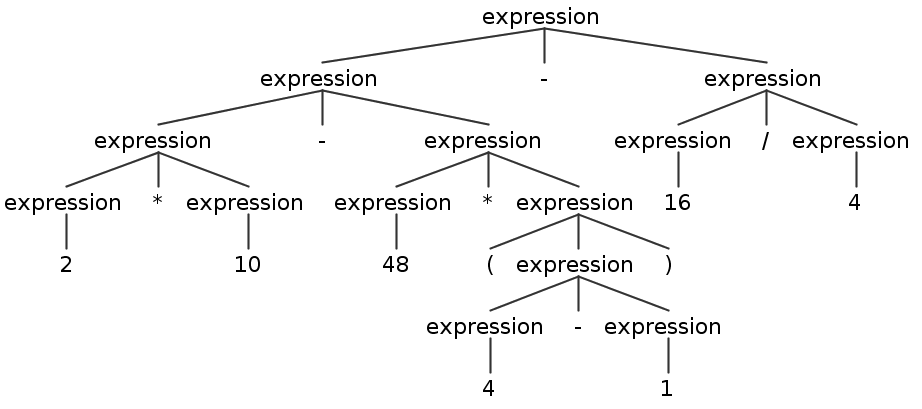
\includegraphics[scale=0.4]{antlr4_parse_tree_arithmetic.png}
\caption{Syntaxbaum für beispielhaften arithmetischen Ausdruck}
\label{fig:method}
\end{figure}

Des Weiteren ist zu beachten, dass arithmetischen Ausdrücke gleicher Operatorenpriorität von links  nach rechts ausgewertet werden müssen. Als Beispiel lässt sich hier der Term 
\begin{lstlisting} [frame=single]
8-5+2
\end{lstlisting}
nennen. Sowohl die Subtraktion als auch die Addition besitzen die gleiche Bindung. Wenn man hier fälschlicherweise zuerst die Addition, also 5+2, was 7 ergibt, auswertet und das Ergebnis dieser Operation von 8 subtrahiert, erhält man als Gesamtergebnis 1. 
In der korrekten Reihenfolge erfolgt zuerst die Subtraktion, also 8-5, was 3 ergibt, und erst darauf die Addition von 1, was als Gesamtergbnis 4 liefert. 
Um diese Fehlerquelle auszuschließen, sind in unserer Grammatik die Regel für Subtraktion vor der für Addition und die Regel für Division vor der für Multiplikation definiert. Da bei reinen Additionen bzw. reinen Multiplikationen die Auswertungsreihenfolge tatsächlich keine Rolle spielt, eine Subtraktion jedoch vor einer Additionen (vgl. Beispiel oben) ausgewertet werden muss, sorgt die Reihenfolge der Regeln in der Grammatik für eine korrekte Auswertung.

Ein analoges Beispiel zu Divisionen und Multiplikationen ist
\begin{lstlisting} [frame=single]
8/2*4
\end{lstlisting}
Auch hier ergibt sich ein ähnliches Problem wie beim vorherigen Beispiel. Wird zuerst die Multiplikation (2*4) ausgeführt und erst danach die Division (also 8/8 in diesem Fall), ist das Endergbnis 1 und nicht wie in der richtigen Reihenfolge 16.

Nach diesen Schritten sind wir also in der Lage einen Syntaxbaum zu erstellen. Der nötige Programmcode dafür wird von ANTLR automatisiert erstellt. Dabei ist die Eingabe dieses Programmes der auszuwertende Ausdruck. Die Ausgabe ist der Syntaxbaum, der zu Testzwecken auch als Grafik (vgl. Abbildung oben) ausgegeben werden kann. 

\pagebreak

Der nächste wichtige Schritt der Übersetzung besteht nun in der Auswertung dieses Baumes. Dazu wird der Baum als Datenstruktur betrachtet. ANTLR liefert dabei mehrere Methoden, die auf Instanzen der Klasse ''ParseTree'' angewandt werden können. 
Jedes Token, das in der Grammatik definiert wurde und durch einen Knoten im Baum repräsentiert wird, besitzt eine sogenannte Visit-Methode. Diese Methode gibt eine Kette mit Zeichen zurück, wobei diese Zeichenkette die Anweisungen in der Zielsprache (Jasmin) enthält. Das Abarbeiten dieser Visit-Methoden in der richtigen Reihenfolge bildet die Grundlage für die Übersetzung, da hiernach alle Instruktionen in der Zielsprache zusammengesetzt sind. Was genau in einer Visit-Methode passiert, wird vom Entwickler festgelegt. ANTLR stellt sogehesen nur eine Vorlage zur Verfügung.

Um diese korrekte Reihenfolge zu gewährleisten, muss eine Anfangsregel (Startaxiom) festgelegt sein. In diesem Beispiel wurde festgelegt, dass der Programmstart - sprich der Wurzelknoten des Baumes - eine ''expression'' sein muss. Das bedeutet, das zunächst die Visit-Methode des Wurzelknoten aufgerufen wird. Damit nun auch die inneren Knoten des Syntaxbaums berücksichtigt werden, ist der Aufruf einer weiteren von ANTLR generierten Methode notwendig. Jeder Knoten des Baum besitzt eine visitChild()-Methode, welche die entsprechenden Visit-Methoden der untergeordneten Knoten aufruft.

Um diese rekursive Vorgehensweise verständlicher zu machen, folgt ein Beispiel.


\begin{lstlisting} [frame=single]
/**@brief
 * verarbeitet Additionen
 */
public String visitAddition(AdditionContext ctx) {
	return visitChildren(ctx) + "\n"
		+ "iadd\n";
}
\end{lstlisting}
Die Tatsache, dass es eine Methode visitAddition mit diesem Eingabeparameter und diesem Rückgabewert gibt, geht auf ANTLR zurück. Der Funktionsrumpf wurde jedoch von uns verfasst.



\subsection{Ausweiten der simplen Grammatik}
Nachdem die Sprache grundlegende Funktionalität erhielt, versuchten wir die weiteren Bestandteile, die durch die Anforderungen festgelegt wurden, zu implementieren. 


\subsection*{Ergebnisausgabe}
Ein Programm ohne Ausgabe ergibt keinen Sinn, da nie das berechnete Ergebnis betrachtet werden kann. Eine Ausgabefunktion zu implementieren stellte sich nicht als all zu großes Problem heraus, da Jasmin die Fähigkeit besitzt Objekte und Methoden in der Java Libary zu nutzen. Wir implentierten dies Ausgabefunktion wie folgt:

\begin{lstlisting}[frame=single]
/**@brief
 * vearbeitet den Aufruf der println-Funktion
 */
public String visitPrintln(PrintlnContext ctx) {
	return  ";calling println\n" + 
		//legt ein System.out Objekt auf den Stack
		"getstatic java/lang/System/out Ljava/io/PrintStream;\n" + 	
		//Argument der print-Funktion
		visit(ctx.argument) + 						
		//ruft die Methode println des System.out-Objekts auf
		"invokevirtual java/io/PrintStream/println(I)V\n\n"; 				
}
\end{lstlisting}

Es wird zuerst ein System.out-Objekt auf den Stack gelegt, danach der auszugebende Wert. Schließlich folgt der Aufruf der Methode println(), die das Argument sowie das System.out-Objekt vom Stack wieder herunternimmt.


Der Aufruf in unserer Programmiersprache lautet: 
\begin{lstlisting}[frame=single]
println( argument );
\end{lstlisting}

\subsection{Implementierung von Variablen}

\subsection{Implementierung von Funktionen}


\subsection{Implementierung von Konstanten}

\subsection{Implementierung von Bedingten Verzweigungen}

\subsection{Implementierung einer Schleife}




\pagebreak
\section{Aufgetrene Probleme und deren Lösung}

\subsection{Operatorenpriorität bei arithmetischen Ausdrücken}

\subsection{Variablen}
Ein wichtiger Bestandteil jeder Programmiersprache ist die Möglichkeit Variablen zu nutzen. Damit eine Variable im späteren Programmverlauf genutzt werden kann, muss sie zunächst deklariert werden. In unserer Sprache erfolgt dies durch die Angabe [Datentyp] [Name];. Beispielsweise legt der Aufruf

\begin{lstlisting}[frame=single]
int x;
\end{lstlisting}

eine Integer-Variable mit dem Namen x an.

Als nächstes sollte eine Wertzuweisung erfolgen:
\begin{lstlisting}[frame=single]
x = 42;
\end{lstlisting}

Nachdem diese obligatorischen Schritte vollzogen wurde, kann der Wert der Variable beliebig oft ausgelesen oder verändert werden.

Damit diese Features in die Zielsprache zu übertragen werden, nutzt unser Compiler eine Variablentabelle. Jasmin besitzt die Möglichkeit den Wert der oben auf dem Stack liegt zwischenzuspeichern. Der Befehl
\begin{lstlisting}[frame=single]
astore <var-num>
\end{lstlisting}
nimmt den Wert vom Stack und speichert in am Index <var-num> in der Variablentabelle.

Mit dem Befehl
\begin{lstlisting}[frame=single]
aload <var-num>
\end{lstlisting}
wird die Variable an der Position <var-nam> wieder auf den Stack gelegt. 
Jasmin akzeptiert nur ganze Zahlen > 0, jedoch keine Zeichenketten, für <var-num>
Deshalb muss unser Compiler den Variablenname, den der Nutzer der Sprache wählt, zu einem Index auflösen.

\subsection*{Redifinition von bereits definierte Variable}
Wenn im Syntaxbaum eine Variablendeklaration gefunden wird, wird zunächst überprüft, ob eine Variable mit diesem Namen bereits vorhanden ist. Für diesen Abgleich wird intern eine HashMap verwendet. Ist der Name noch nicht vorhanden, wird er der HashMap hinzugefügt, wobei der Schlüssel der Name der Variable und der Wert die aktuelle Größe der Tabelle ist. Dies ist notwendig, um den Jasmin-Befehlen astore und aload einen Index  zu übergeben.

\subsection*{Zugriff auf undefinierte Variable}
Ein möglicher Fehler seitens des Benutzer unserer Sprache ist, dass eine Variable aufgerufen wird, obwohl diese zuvor nicht definiert wurde. Beim Aufruf einer Variablen wird deshalb zunächst überprüft, ob diese in der Variablen-Map vorhanden ist. Falls nicht wird eine entsprechende Exception ausgelöst.


\subsection{Funktionen}
\subsection*{Zugriff auf undefinierte Funktion}
\subsection*{Redifinition von bereits defnierter Funktion}
\subsection*{Gültigkeitsbereiche}
\subsection*{Funktionen mit gleichem Namen und unterschiedlichen Signaturen}
\subsection*{Vorwärtsdeklarationen}

\subsection{Bedingte Verzweigungen}
\subsection*{Umsetzung in Jasmin mit Hilfe von Labels und Sprungbefehlen}



\pagebreak
\section{Verwendung des Compilers}
Abbreviations should be introduced at the first mention in the main text – no abbreviations lists. Suggested structure of main text (not enforced) is provided below.
Must include all authors, identified by initials, for example:
A.A. conceived the experiment(s),  A.A. and B.A. conducted the experiment(s), C.A. and D.A. analysed the results.  All authors reviewed the manuscript.

\section*{Additional information}

To include, in this order: \textbf{Accession codes} (where applicable); \textbf{Competing interests} (mandatory statement).

The corresponding author is responsible for submitting a \href{http://www.nature.com/srep/policies/index.html#competing}{competing interests statement} on behalf of all authors of the paper. This statement must be included in the submitted article file.

\begin{figure}[ht]
\centering
\includegraphics[width=\linewidth]{/home/noah/Pictures/meisterwerk.jpg}
\caption{Legend (350 words max). Example legend text.}
\label{fig:stream}
\end{figure}

\begin{table}[ht]
\centering
\begin{tabular}{|l|l|l|}
\hline
Condition & n & p \\
\hline
A & 5 & 0.1 \\
\hline
B & 10 & 0.01 \\
\hline
\end{tabular}
\caption{\label{tab:example}Legend (350 words max). Example legend text.}
\end{table}

Figures and tables can be referenced in LaTeX using the ref command, e.g. Figure \ref{fig:stream} and Table \ref{tab:example}.


\section{Anhang}
\subsection{Quellenangaben}

\subsection{Quellcode des Compiler(?)}


\end{document}
